\chapter{Genealogía de Procesos en Windows}

La genealogía de procesos en Windows representa la jerarquía de creación de
procesos desde el arranque del sistema hasta el inicio de sesión del usuario.
Comprender esta estructura es esencial para el análisis forense, la respuesta a
incidentes y la detección de malware, ya que permite identificar comportamientos
anómalos en los procesos del sistema.

\section*{Nivel 0: Proceso raíz}

\begin{itemize}
    \item \textbf{System}: Primer proceso de espacio de usuario iniciado por el
    kernel. Tiene un PID fijo (normalmente 4) y no tiene padre.
\end{itemize}

\section*{Nivel 1: Session Manager}

\begin{itemize}
    \item \textbf{smss.exe (Session Manager Subsystem)}: Primer proceso real del
    espacio de usuario. Se encarga de iniciar las sesiones del sistema, lanzar
    procesos críticos como \texttt{csrss.exe}, \texttt{wininit.exe} y
    \texttt{winlogon.exe}.
\end{itemize}

\section*{Nivel 2: Procesos críticos del sistema}

\begin{itemize}
    \item \textbf{csrss.exe}: Client/Server Runtime Subsystem. Se encarga de
    funciones esenciales como la gestión de la consola y la creación de
    procesos. Existe una instancia por sesión.
    \item \textbf{wininit.exe}: Windows Initialization Process. Lanza procesos
    esenciales como \texttt{services.exe}, \texttt{lsaiso.exe} y
    \texttt{lsass.exe}.
    \item \textbf{winlogon.exe}: Gestiona la autenticación del usuario y se
    mantiene activo durante la sesión interactiva.
\end{itemize}

\section*{Nivel 3: Procesos del sistema}

\begin{itemize}
    \item \textbf{services.exe}: Service Control Manager. Se encarga de iniciar
    y gestionar los servicios del sistema, incluyendo los alojados por
    \texttt{svchost.exe}.
    \item \textbf{lsaiso.exe}: Proceso de seguridad aislado que implementa
    funciones de cifrado y autenticación en versiones modernas de Windows
    (opcional).
    \item \textbf{lsass.exe}: Local Security Authority Subsystem Service.
    Encargado de políticas de seguridad, autenticación y gestión de
    credenciales.
\end{itemize}

\section*{Nivel 4: Servicios alojados y utilidades del sistema}

\begin{itemize}
    \item \textbf{svchost.exe}: Proceso contenedor que aloja múltiples servicios
    del sistema. Existen muchas instancias según el grupo de servicios que
    aloje.
    \item \textbf{runtimebroker.exe / taskhostw.exe}: Procesos auxiliares para
    la ejecución de aplicaciones y tareas programadas.
\end{itemize}

\section*{Procesos del usuario interactivo}

\begin{itemize}
    \item \textbf{userinit.exe}: Iniciado por \texttt{winlogon.exe} tras la
    autenticación. Lanza el shell principal del usuario y termina.
    \item \textbf{explorer.exe}: Shell gráfico de Windows que representa el
    escritorio, la barra de tareas y el menú de inicio. Es el proceso raíz del
    entorno del usuario.
\end{itemize}

\section*{Importancia en Ciberseguridad}

Comprender esta estructura es fundamental para:
\begin{itemize}
    \item Identificar procesos anómalos o fuera de lugar.
    \item Detectar técnicas de evasión como \textit{Process Injection} o
    \textit{Parent PID Spoofing}.
    \item Realizar análisis forense de procesos mediante herramientas como
    Sysmon, EDR, Process Explorer, o Zeek.
\end{itemize}

\vspace{1em}
\noindent A continuación se muestra la genealogía de procesos típica en
Windows:

\begin{center}
    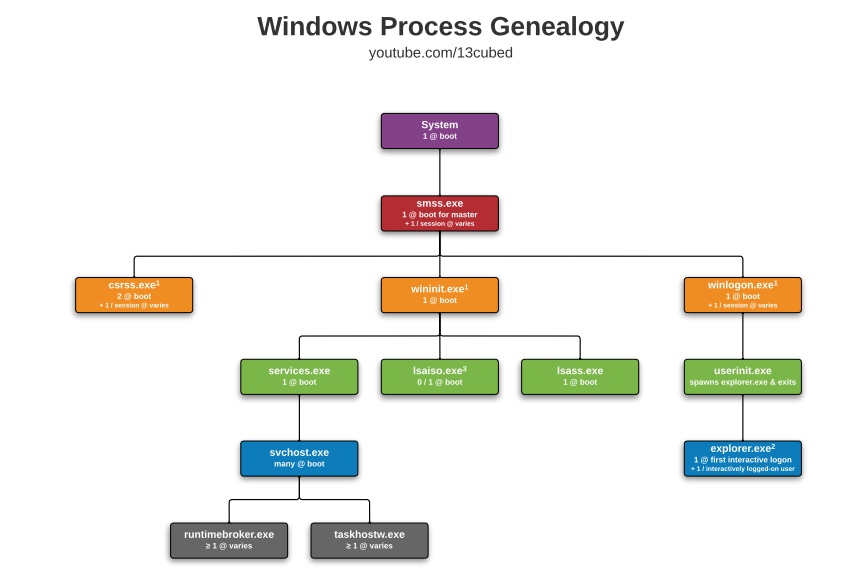
\includegraphics[width=0.95\textwidth]{image.png}
\end{center}

\noindent Fuente: \texttt{youtube.com/13cubed}

